% =============================================================================
\section{Phase noise}
% =============================================================================

Another important characteristic of a \abbrev{bec} interferometry experiment is the phase noise, which is connected with the visibility.
We will discuss it based on the same experiment~\cite{Egorov2011,Egorov2012} as in the previous section.

While in the simulation we can measure the visibility~\eqnref{bec-noise:visibility:visibility} simply by calculating a second-order moment, experimentalists do not have the luxury of knowing the wavefunctions of the components.
Instead, multiple runs of the Ramsey sequence with the same evolution time are performed, with the second $\pi/2$-pulse having a different phase lag $\phi$ each time.
The quantity that can be measured in the experiment is the normalized atom difference
\begin{eqn}
    P_z = \frac{N_2^\prime - N_1^\prime}{N_1^\prime + N_2^\prime},
\end{eqn}
where $N_1^\prime$ and $N_2^\prime$ are populations of the components obtained by imaging after the second $\pi/2$-pulse.
Using the rotation matrix~\eqnref{bec-noise:mean-field:rotation-matrix} it can be shown that $P_z$ can be expressed in terms of wave operators before the second $\pi/2$-pulse as
\begin{eqn}
    P_z(\phi)
    = - \frac{2}{N_1 + N_2} \Imag \left(
        e^{-i\phi} \int \langle \Psiop_1^\dagger \Psi_2 \rangle \upd\xvec
        \right).
\end{eqn}
One can notice that the integral of the second order moment in this expression is the same as in~\eqnref{bec-noise:visibility:visibility}, and is also normalized on the total population.
Therefore if we vary $\phi$ in the experiment, the resulting $P_z(\phi)$ can be fit with a sine function, and its amplitude will give us the visibility $\mathcal{V}$.

\begin{figure}
    \centerline{%
    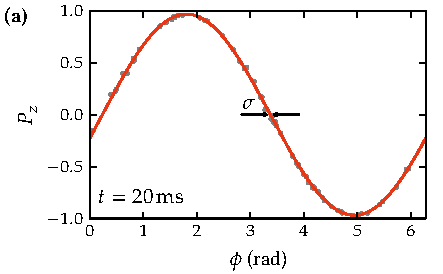
\includegraphics{figures_generated/bec_noise/illustration_noise_20ms.pdf}%
    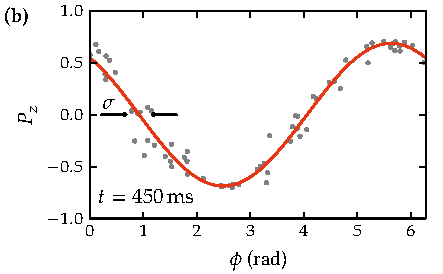
\includegraphics{figures_generated/bec_noise/illustration_noise_450ms.pdf}}

    \caption{Phase noise in experimental measurements of visibility at \textbf{(a)}~$t = 20\un{ms}$ and \textbf{(b)}~$t = 450\un{ms}$.
    Black dots illustrate possible results obtained in a single run of the Ramsey interferometry experiment.}%endcaption

    \label{fig:bec-noise:phase-noise:illustration}
\end{figure}

In practice, naturally, the measurement of $P_z$ is affected by various sources of technical noise.
As a result, the measured points are displaced from the ideal curve.
In the experiment in question three such noise sources were identified.
First, the length of $\pi/2$-pulses varied throughout the exeprimental runs with an estimated standard deviation of $\Delta \theta = 0.02\un{rad}$ (caused by the drift of the Rabi frequency $\Omega$).
The phase of the coupler also had an uncertainty caused by the MW frequency instability that grew with time as $\Delta \phi / t = 0.5\un{rad/s}$.
Finally, the imaging technique used to measure populations $N_1^\prime$ and $N_2^\prime$ resulted in an uncertainty of $\Delta N / N = 0.023$.
These factors can be trivially added to the simulations: first two at the moment of the application of the rotation matrix~\eqnref{bec-noise:mean-field:rotation-matrix}, by adding a random factor to the length $\theta$ and the phase $\phi$, and the third one by adding a random factor to the populations $N_1$ and $N_2$ produced by integrating the corresponding moments of wavefunctions.

The result is is illustrated in~\figref{bec-noise:phase-noise:illustration}, with the ``experimental'' points emulated this way plotted agains a sine fit, for two different evolution times.
The base simulation is the truncated Wigner one for the regular Ramsey sequence from the previous section.
The standard deviation of the horizontal distance $\sigma$ of the experimental results from the fitting curve is called the phase noise.
The amplitude of the curve, in turn, is taken to be the predicted visibility accounting for the technical noises (see~\figref{bec-noise:visibility:ramsey-visibility} and~\figref{bec-noise:visibility:echo-visibility} in the previous section).

\begin{figure}
    \centerline{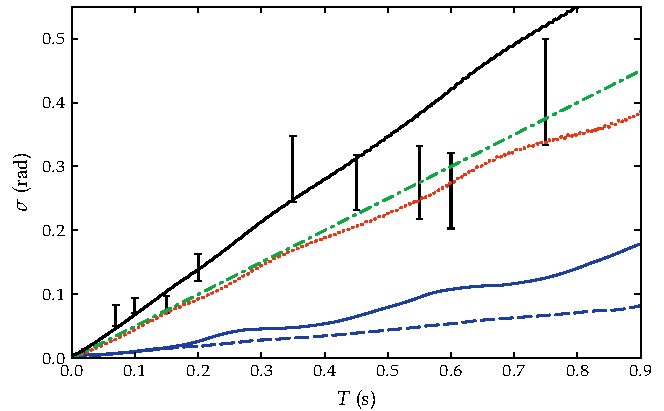
\includegraphics{figures_generated/bec_noise/ramsey_noise.pdf}}

    \caption{Comparison of experimental (black bars) and numerically simulated phase noise at the end of a Ramsey sequence with the evolution time $t$.
    The truncated Wigner predictions with (blue solid line) and without (red dashed line) the inclusion of technical noises is shown.}%endcaption

    \label{fig:bec-noise:phase-noise:ramsey-phnoise}
\end{figure}

A comparison of the phase noise with the experimental data for the regular Ramsey sequence is shown in~\figref{bec-noise:phase-noise:ramsey-phnoise}.
The experimental parameters are the same as in the previous section.
The effect of quantum noise (red dashed line) is noticeable, but not very large as compared to the compound effect of the technical noises (blue solid line).
There seems to be a lot of room for the improvement of the apparatus until the measurements hit the ``hard'' limit of the quantum noise.

\begin{figure}
    \centerline{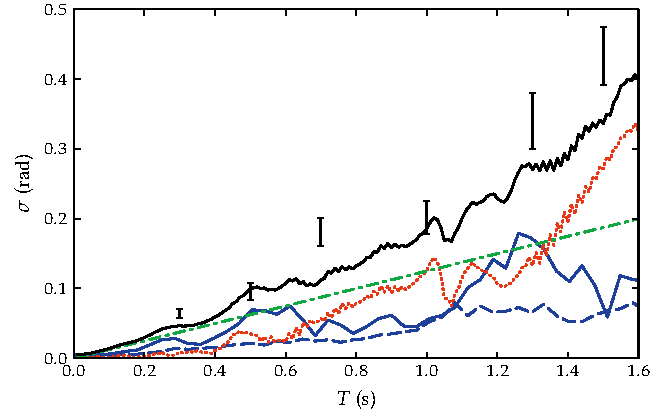
\includegraphics{figures_generated/bec_noise/echo_noise.pdf}}

    \caption{Comparison of experimental (black bars) and numerically simulated phase noise at the end of a spin echo sequence with the evolution time $t$.
    The truncated Wigner predictions with (blue solid line) and without (red dashed line) the inclusion of technical noises is shown.}%endcaption

    \label{fig:bec-noise:phase-noise:echo-phnoise}
\end{figure}

Phase noise in a spin echo sequence can be estimated in the same way.
The reported MW frequency instability for this experiment was $\Delta \phi / t = 0.125\un{rad/s}$.
As~\figref{bec-noise:phase-noise:echo-phnoise} shows, even after the inclusion of the technical noise, there is some disagreement with the experimental data.
This may be caused by the systematic error introduced by the truncation, or possibly by some additional source of technical noise.

One may notice that the total noise shown in~\figref{bec-noise:phase-noise:ramsey-phnoise} and~\figref{bec-noise:phase-noise:echo-phnoise} is lower than the one reported by Egorov \textit{et al}~\cite{Egorov2011,Egorov2012}.
This is the result of the honest calculation of the total noise (in essence, we simulate the actual experimental measurement procedure), as opposed to the post-factum combination of noise from the technical sources with the Wigner results.
